\documentclass[12pt]{extarticle}
\usepackage[utf8]{inputenc}
\usepackage{mathtools}
\usepackage{amsthm}
\usepackage{amsfonts}
\usepackage{tikz}
\usepackage{tkz-berge}
\usepackage{hyperref}
\usepackage{float}
\usepackage[ruled,vlined]{algorithm2e}
\usepackage{todonotes}

\theoremstyle{definition}
\newtheorem{definition}{Definition}[section]
\theoremstyle{remark}
\newtheorem{note}[definition]{Note}
\theoremstyle{plain}
\newtheorem{theorem}[definition]{Theorem}
\theoremstyle{plain}
\newtheorem{lemma}[definition]{Lemma}
\newtheorem{proposition}[definition]{Proposition}
\theoremstyle{plain}
\newtheorem{corollary}[definition]{Corollary}

\newcommand{\BO}{\mathcal{O}}
\newcommand{\E}{\mathbb{E}}

\title{AuW Recap}
\author{
    Axel Montini
    \\
    \href{mailto:amontini@student.ethz.ch}{amontini@student.ethz.ch}
}

\begin{document}
\maketitle

Cannot be used during the exam, but it's a nice short recap of everything done in the second semester.

\section{Last semester}
Go read again about MST algorithms and so on.

\section{Graphentheorie}

\subsection{Zusammenhang}
\begin{definition}
    A graph $G=(V,E)$ is \textit{k-zusammenhängend} if $|V| \ge k + 1$ and
    for all $X \subseteq V,\ |X| < k$ the following is true:
    \[ \mbox{The graph}\ G[V \setminus X]\ \mbox{is zusammengehängend} \]
\end{definition}

\begin{definition}
    A graph $G=(V,E)$ is \textit{k-kanten-zusammenhängend} if
    for all $X \subseteq E,\ |X| < k$ the following is true:
    \[ \mbox{The graph}\ G(V, E \setminus X)\ \mbox{is zusammengehängend} \]
\end{definition}

\begin{note}
    A graph can be both 2-kanten-zusammengehängend and be only 1-zusammengehängend at the same time.
    Example:
    \begin{figure}[H]
        \centering

        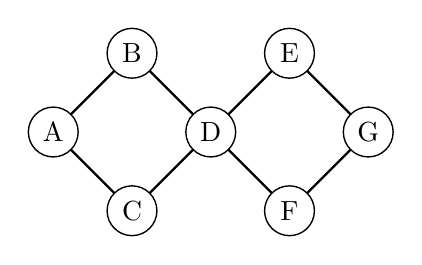
\begin{tikzpicture}
            \Vertex[x=0,y=0]{A}
            \Vertex[x=1,y=1]{B}
            \Vertex[x=1,y=-1]{C}
            \Vertex[x=2,y=0]{D}
            \Vertex[x=3,y=1]{E}
            \Vertex[x=3,y=-1]{F}
            \Vertex[x=4,y=0]{G}

            \Edges(A, B)
            \Edges(A, C)
            \Edges(C, D)
            \Edges(B, D)
            \Edges(D, E)
            \Edges(D, F)
            \Edges(E, G)
            \Edges(F, G)
        \end{tikzpicture}
    \end{figure}
\end{note}

\begin{definition}
    In a zusammengehängend Graph,
    \textit{Artikulationsknoten} disconnect the graph when removed.
    Only 1-zusammengehängend graphs can have Artikulationsknoten
\end{definition}

\begin{theorem}
    In zusammenhängende Graphs it's possible to find Artikulationsknoten in $\BO(|E|)$ if an adjacency list is used.
\end{theorem}

\begin{definition}
    A zusammenhängend Graph may contain \textit{Brücke}. In this case, it's \textbf{not 2-kanten-zusammenhängend}.

    An edge is a bridge if it disconnects the graph when removed.
\end{definition}

\begin{theorem}
    Brücke can also be computed in $\BO(|E|)$ using an adjacency list.
\end{theorem}

\begin{definition}
    $G = (V,E)$ is zusammenhängend. For $e,f \in E$ we define the relation
    \[ e \sim f \Leftrightarrow e = f\ \mbox{or there is a Kreis containing both edges} \]

    This is an equivalence relation. Each equivalence class is called a \text{Block} (plural \text{Blöcke}).
\end{definition}

\subsection{Kreise}

\begin{definition}
    An \textit{Eulertour} in a graph $G$ is a closed path (\textit{Zyklus}) that contains every edge $\in E$ exactly once.

    A graph containing an Eulertour is called \textit{eulersch}.
\end{definition}

\begin{definition}

\end{definition}

\begin{theorem}
    \[ \mbox{A graph is eulersch} \Leftrightarrow deg(v)\ \mbox{is even for all vertices}\]
\end{theorem}

\begin{theorem}
    In a connected and eulersch Graph it's possible to find an Eulertour in $\BO(|E|)$.
\end{theorem}

\begin{definition}
    A \textit{Hamintonkreis} in $G$ is a cycle that goes through every vertex exaclty once.
    A graph containing an Hamintonkreis is called \textit{hamintonsch}.
\end{definition}

\begin{theorem}
    The algorithm seen in class can find an Hamintonkreis in time $\BO(n^2 \cdot 2^n)$ and memory $\BO(n \cdot 2^n)$, where $n = |V|$.
\end{theorem}

\begin{theorem}
    A bipartite graph $G = (A \uplus B, E)$ cannot contain an Hamintonkreis.
\end{theorem}

\begin{theorem}[Dirac]
    A graph $G$ with $V \ge 3$ in which every vertex has at least $|V|/2$ neighbors is \textit{hamintonsch}.
\end{theorem}

\begin{definition}
    In a complete graph $K_n$ (all vertices are connected together),
    the metric Traveling Salesman Problem consists in finding an
    Hamintonkreis $C$ with minimal cost (distance).
\end{definition}

\begin{definition}
    An $\alpha$-Approximationsalgorithmus of this problem finds an H.kreis $C$ so that
    \[ \sum_{e \in C} l(e) \le \alpha \cdot opt(K_n, l) \]
    Meaning that it finds a solution worse by the optimal solution by a factor $\alpha$.
\end{definition}

\begin{theorem}
    If there's an $\alpha$-Approximationsalgorithmus with $\alpha > 1$ for the TSP with running time $\BO(f(n))$ then there's
    also an algorithm that decides whether a graph with $n$ vertices is hamintonsch in $\BO(f(n))$.
\end{theorem}
\begin{theorem}
    For the metric TSP there's a 2-Approximationsalgorithmus with running time $\BO(n^2)$.
    It find the MST in $\BO(n^2)$ and then uses it to find the H.k.
\end{theorem}

\subsection{Matching}

\begin{definition}
    A set of edges $M \subseteq E$ is called \textit{Matching} in a graph $G$ if
    \[ \forall e,f \in M\ (e \cap f = \emptyset) \]

    \begin{itemize}
        \item A vertex $v$ is said to be \textit{überdeckt} by a matching $M$ if the matching contains an edge containing $v$.
        \item A matching $M$ is called \textit{perfektes Matching} if every vertex is überdeckt (equivalent: $|M| = |V| / 2$).
    \end{itemize}
\end{definition}

\begin{definition}
    A matching $M$ is said to be:
    \begin{itemize}
        \item \textit{inklusionsmaximal} if $M \cup \left\{ e \right\}$ is not a matching for all $e \in E \setminus M$.
        \item \textit{kardinalitätsmaximal} if $|M| \ge |M'|$ for all matchings $M'$ in $G$.
    \end{itemize}

    Note that \textit{kardinalitätsmaximal} $\Rightarrow$ \textit{inklusionsmaximal} (the opposite might not be true).
\end{definition}

\begin{theorem}
    \begin{algorithm}
        \caption{Greedy-Matching}
        \KwResult{The inklusionsmaximales matching $M$}
        \While{$E \ne \emptyset$}{
            choose an edge $e \in E$\;
            $M \gets M \cup \left\{ e \right\}$\;
            remove $e$ and all incident edges from $G$\;
        }
    \end{algorithm}

    The greedy-matching algorithm finds an inklusionsmaximal Matching in time $\BO(|E|)$
    for which the following holds: $|M_{Greedy}| \ge \frac{1}{2} |M_{max}|$, where $M_{max}$ is a kardinalitätsmaximales Matching.
\end{theorem}

\begin{theorem}[Berge]
    Let $M$ be a matching in $G$ that is not k.maximal, then there is an augmenting path to $M$.
    \todo{Algos at page 65 and 67}
\end{theorem}

\begin{theorem}
    Is $n$ even $K_n$ a complete graph, then it's possible to find a \textit{minimal perkeftes Matching} in time $\BO(n^3)$
\end{theorem}

\begin{theorem}
    There's a 3/2-Approximationsalgorithmus for the TSP that runs in $\BO(n^3)$.
\end{theorem}

\begin{definition}
    \textit{Nachbarnschaft einer Knotenmenge} $X \subseteq V$:
    \[ N(X) := \bigcup_{v \in X} N(v) \]
\end{definition}

\begin{theorem}[Hall, Heiratssatz]
    For a bipartite graph $G = (A \uplus B, E)$ theres a matching $M$ with $|M| = |A|$ if and only if $|N(X)| \ge |X|$ for all $X \subseteq A$.
\end{theorem}

\begin{definition}
    A bipartite graph is called \textit{k-regulär} if every vertex has degree $k$.
\end{definition}

\begin{theorem}
    Let $G$ be a k-regular bipartite graph. Then there's $M_1, ..., M_k$ so that $E = M_1 \uplus M_2 \uplus ... \uplus M_k$ and all
    $M_i, 1 \le i \le k$ are perfect matchings.
\end{theorem}

\begin{theorem}
    Is $G = (V, E)$ a $2^k$-regular bipartite Graph, then it's possible to find a perfect matching in $\BO(|E|)$.
\end{theorem}

\subsection{Färbungen}

\begin{definition}
    A \textit{(Knoten)-Färbung} (vertex coloring) of a graph $G$ with $k$ colors is $c: V \to [k]$, so that
    \[ c(u) \ne c(v)\ \forall \left\{ u, v \right\} \in E \]

    The \textit{chromatische Zahl} (chromatic number) $X(G)$ of a graph is the minimal amount of colors that can be used to
    color $G$.
\end{definition}

\begin{theorem}
    A graph is bipartite if and only if doesn't contain any Kreis of odd length.
\end{theorem}

\begin{theorem}[Vierfarbensatz]
    Every map can be colored with 4 colors.
\end{theorem}

\begin{theorem}
    \begin{algorithm}
        \caption{Greedy-Färbung}
        \KwData{$G$}
        \KwResult{array $c$ mapping each vertex to a color}
        $c(v_1) \gets 1$\;
        \For{$i = 2, \dots, n$}{
            $c(v_i) \gets \min \left\{ k \in \mathbb{N} \mid k \ne c(u)\ \mbox{for all}\ u \in N(v_i) \cap \left\{ v_1, ..., v_{i - 1} \right\} \right\}$
        }
    \end{algorithm}

    Let $G$ be a connected graph and $C(G)$ the amount of colors used by the Greedy-Färbung algorithm.
    Then
    \[ \mathcal{X}(G) \le C(G) \le \Delta(G) + 1 \]
    Where $\Delta(G) := \max_{v \in V} deg(v)$ is the max degree in the graph.

    The running time is $\BO(|E|)$ if an adjacency list is used.
\end{theorem}

\begin{theorem}[Brooks]
    Let $G$ be a connected graph that is neither complete nor an odd Kreis ($G \ne K_n$ and $G \ne C_{2n+1}$).
    Then
    \[ \mathcal{X}(G) \le \Delta(G) \]
    And there's an algorithm that can color the vertices of $G$ in time $\BO(|E|)$ and with $\Delta(G)$ colors.
\end{theorem}

\begin{theorem}[Mycielski-Konstruktion]
    For all $k \ge 2$ there's a triangle-free graph $G_k$ with $\mathcal{X}(G) \ge k$.
\end{theorem}

\begin{theorem}
    Every 3-färbbaren graph can be colored in time $\BO(|E|)$ with $\BO(\sqrt{|V|})$ colors.
\end{theorem}

\section{Randomized algorithms}

\subsection{Grundbegriffe und Notationen}

\begin{definition}
    A \textit{diskreter Wahrscheinlichkeitsraum} is defined through a \textit{Ergebnismenge}
    $\Omega = \left\{ \omega_1, \omega_2, ... \right\}$ of \textit{Elementarereignissen}.

    A probability $\Pr[\omega_i]$ corresponds to each $\omega_i$.
    \[0 \le \Pr[w_i] \le 1,\quad \sum_{\omega \in \Omega} \Pr[\omega] = 1\]

    A set $E \subseteq \Omega$ is called \textit{Ereignis}. The probability is defined as
    \[ \Pr[E] := \sum_{\omega \in E} \Pr[\omega] \]

    The \textit{Komplementärereignis} zu $E$ is defined as $\overline{E} := \Omega \setminus E$
\end{definition}

\begin{lemma}
    For \textit{Ereignisse} $A,B$:
    \begin{enumerate}
        \item $\Pr[\emptyset] = 0, \Pr[\Omega] = 1$
        \item $0 \le \Pr[A] \le 1$
        \item $\Pr[\overline{A}] = 1 - \Pr[A]$
        \item If $A \subseteq B$ then $\Pr[A] \le \Pr[B]$
    \end{enumerate}
\end{lemma}

\begin{theorem}[Additionssatz]
    When the \textit{Ereignisse} are pairwise disjoint then
    \[ \Pr \left[ \bigcup_{i=1}^n A_i \right] = \sum_{i=1}^n \Pr[A_i] \]
    For infinite sets of disjoint Ereignissen $A_1, A_2, ...$ then
    \[ \Pr \left[ \bigcup_{i=1}^\infty A_i \right] = \sum_{i=1}^\infty \Pr[A_i] \]
\end{theorem}

\begin{theorem}[Siebformel, Prinzip der Inklusion/Exklusion]
    For Ereignisse $A_1, ..., A_n \ (n \ge 2)$:
    \[ \Pr \left[ \bigcup_{i=1}^n A_i \right] = \sum_{l=1}^n (-1)^{l+1} \sum_{1 \le i_1 < ... < i_l \le n} \Pr[A_{i_1} \cap ... \cap A_{i_l}] \]
\end{theorem}

\begin{lemma}[A special case of the Siebformel]
    Let $\Omega = A_1 \cup ... \cup A_n$ with $\Pr[\omega] = 1/|\Omega|$,
    where $A_i$ are finite sets.
    Then
    \[ | \bigcup_{i=1}^n A_i | = \sum_{l=1}^n (-1)^{l+1} \sum_{1 \le i_1 < ... < i_l \le n} |A_{i_1} \cap ... \cap A_{i_l}| \]
\end{lemma}

\begin{corollary}[Boolsche Ungleichung, Union Bound]
    For some Ereignisse $A_1, ..., A_n$:
    \[ \Pr \left[ \bigcup_{i=1}^n A_i \right] \le \sum_{i=1}^n \Pr[A_i]\]
    For an infinite set of Ereignisse, replace $n$ with $\infty$.
\end{corollary}

\subsection{Bedingte Wahrscheinlichkeiten}

\begin{definition}
    Let $A$ and $B$ be Ereignisse with $\Pr[B] > 0$.
    The \textit{bedingte Wahrscheinlichkeit} $Pr[A|B]$ of $A$ given $B$
    is defined through
    \[ \Pr[A|B] := \frac{\Pr[A \cap B]}{\Pr[B]} \]
\end{definition}

\begin{theorem}[Multiplikationssatz]
    The Ereignisse $A_1, ..., A_n$ are given.
    If $\Pr[A_1 \cap ... \cap A_n] > 0$, then:
    \[ \Pr[A_1 \cap ... \cap A_n] = \Pr[A_1] \cdot \Pr[A_2 | A_1] \cdot \Pr[A_3 | A_1 \cap A_2] \cdot ... \cdot \Pr[A_n | A_1 \cap ... \cap A_{n-1}] \]
\end{theorem}

\begin{theorem}[Satz von der totalen Wahrscheinlichkeit]
    $A_1, ..., A_n$ are pairwise disjoint and $B \subseteq A_1 \cup ... \cup A_n$.
    Then
    \[ \Pr[B] = \sum_{i=1}^n \Pr[B|A_i] \cdot \Pr[A_i] \]
    Analogous for an infinite set of $A_i$s.
\end{theorem}

\begin{theorem}[Satz von Bayes]
    $A_1, ..., A_n$ pairwise disjoint.
    Let $B \subseteq A_1 \cup ... \cup A_n$ with $\Pr[B] > 0$.
    Then for any $i = 1,...,n$:
    \[ \Pr[A_i | B] = \frac{\Pr[A_i \cap B]}{\Pr[B]} = \frac{\Pr[B|A_i] \cdot \Pr[A_i]}{\sum_{j=1}^n \Pr[B|A_j] \cdot \Pr[A_j]} \]

    Analogous for $\infty$ instead of $n$.
\end{theorem}

\subsection{Unabhängigkeit}

\begin{definition}
    Die Ereignisse $A, B$ are \textit{unabhängig} when
    \[ \Pr[A \cap B] = \Pr[A] \cdot \Pr[B] \]
\end{definition}

\begin{definition}
    Die Ereignisse $A_1, ..., A_n$ are unabhängig when for all $I \subseteq \left\{ 1, ..., n \right\}$
    with $I = {i_1, ..., i_k}$:
    \[ \Pr \left[ A_{i_1} \cap ... \cap A_{i_k} \right] = \Pr \left[ A_{i_1}] \cdot ... \cdot \Pr[A_{i_k} \right] \]
\end{definition}

\begin{lemma}
    Die Ereignisse $A_1, ..., A_n$ are unabängig \textbf{if and only if}
    \[ \forall (s_1, .., s_n) \in \left\{ 0, 1 \right\}^n\ \left( \Pr[A_1^{s_1} \cap ... \cap A_n^{s_n}] = \Pr[A_1^{s_1}] \cdot \Pr[A_n^{s_n}] \right) \]
    where $A_i^0 = \overline{A_i}$ and $A_i^1 = A_i$
\end{lemma}

\begin{lemma}
    $A, B, C$ unabängige Ereignisse.
    Then $A \cap B$ and $C$ and $A \cup B$ and $C$ are also independent.
\end{lemma}

\subsection{Zufallsvariablen}

\begin{definition}
    A \textit{Zufallsvariable} is $X:\Omega \to \mathbb{R}$,
    where $\Omega$ is the Ergebnismenge of a Wahrscheinlichkeitsraum.

    The \textit{Wertebereich} of a Zufallsvariable is
    \[ W_X := X(\Omega) = \left\{ x \in \mathbb{R} \mid \exists \omega \in \Omega\ \mbox{with}\ X(\omega) = x \right\} \]
\end{definition}

\begin{definition}
    The \textit{Erwartungswert} of $X$ is $\E[X]$, defined as
    \[ \E[X] := \sum_{x \in W_x} x \cdot \Pr[X = x] \]
    when the sum absolut konvergiert. Otherwise the Erwartungswert is \textit{undefiniert / undefined}.
\end{definition}

\begin{lemma}
    Is $X$ a Zufallsvariable, then:
    \[ \E[X] = \sum_{\omega \in \Omega} X(\omega) \cdot \Pr[\omega] \]
\end{lemma}

\begin{theorem}
    $X$ Zufallsvariable wit $W_X \subseteq \mathbb{N}_0$. Then
    \[ \E[X] = \sum_{i=1}\infty \Pr[X \ge i] \]
\end{theorem}

\begin{theorem}
    $X$ a Zufallsvariable. For pairwise disjoint Ereignisse $A_1, ..., A_n$ with $A_1 \cup ... \cup A_n = \Omega$ and
    $\Pr[A_1],...,\Pr[A_n] > 0$ then
    \[ \E[X] = \sum_{i=1}^n \E[X | A_i] \cdot \Pr[A_i] \]

    Analogous for $\infty$ instead of $n$.
\end{theorem}

\begin{theorem}[Linearität des Erwartungswert]
    For $X_1, ..., X_n$ and $X := a_1 X_1 + ... + a_n X_n + b$ with $a_1, ..., a_n, b \in \mathbb{R}$:
    \[ \E[X] = a_1 \E[X_1] + ... + a_n \E[X_n] + b \]
\end{theorem}

\begin{note}
    For an Ereignis $A \subseteq \Omega$ the \textit{Indikatorvariable} $X_A$ is defined as
    \[ X_A(\omega) := \begin{cases}
            1, & \mbox{if}\ \omega \in A \\
            0, & \mbox{otherwise}        \\
        \end{cases} \]

    Also $\E[X_A] = \Pr[A]$
\end{note}

\begin{definition}
    For a Zufallsvariable $X$ mit $\mu = \E[X]$ the \textit{Varianz} $Var[X]$ is defined through
    \[ Var[X] := \E[(X - \mu)^2] = \sum_{x \in W_X} (x - \mu)^2 \Pr[X = x] \]

    The \textit{Standardabweichung} of $X$ is $\sigma := \sqrt{Var[X]}$.
\end{definition}

\begin{theorem}
    For any Zufallsvariable $X$ and $a,b \in \mathbb{R}$:
    \[ Var[X] = \E[X^2] - \E[X]^2 \]
    \[ Var[a \cdot X + b] = a^2 \cdot Var[X] \]
\end{theorem}

\begin{definition}
    For a Zufallsvariable $X$, $\E[X^k]$ is called \textit{$k$-te Moment} and
    $\E[(X - \E[X])^k]$ is called \textit{$k$-te zentrale Moment}.
\end{definition}

\subsection{Wichtige diskrete Verteilungen}

\todo{Maybe write, or use the Formelsammlung}
Bernoulli, Binomial, Geometrische, Poisson

\subsection{Mehrere Zufallsvariablen}

\begin{definition}
    Zufallsvariablen $X_1, ..., X_n$ are \textit{unabhängig} if and only if
    for all $(x_1, ..., x_n) \in W_{X_1} \times ... \times W_{X_n}$ the following holds:
    \[ \Pr[X_1 = x_1, ..., X_n = x_n] = \Pr[X_1 = x_1] \cdot ... \cdot \Pr[X_n = x_n] \]
\end{definition}

\begin{theorem}[Linearität des Erwartungswerts]
    For $X_1, ..., X_n$ and $X := a_1 X_1 + ... + a_n X_n$ with $a_i \in \mathbb{R}$:
    \[ \E[X] = a_1 \E[X_1] + ... + a_n \E[X_n] \]
\end{theorem}

\begin{theorem}[Multiplikativität des Erwartungswerts]
    For $X_1, ..., X_n$:
    \[ \E[X_1 \cdot ... \cdot X_n] = \E[X_1] \cdot ... \cdot \E[X_n] \]
\end{theorem}

\begin{theorem}
    For independent $X_1, ..., X_n$ and $X := X_1 + ... + X_n$ then
    \[ Var[X] = Var[X_1] + ... + Var[X_n] \]
\end{theorem}

\subsection{Abschätzen von Wahrscheinlichkeiten}

\begin{theorem}[Ungleichung von Markov]
    $X \ge 0$ Zufallsvariable. Then, for all $t > 0 \in \mathbb{R}$:
    \[ \Pr[X \ge t] \le \frac{\E[X]}{t}\ \mbox{und}\ \Pr[X \ge t \cdot \E[X]] \le \frac{1}{t} \]
\end{theorem}

\begin{theorem}[Ungleichung von Chebyshev]
    $X$ Zufallsvariable and $t > 0 \in \mathbb{R}$. Then
    \[ \Pr[|X - \E[X]| \ge t] \le \frac{Var[X]}{t^2} \]
\end{theorem}

\begin{theorem}[Ungleichung von Chernoff]
    $X_1, ..., X_n$ independent Beroulli-verteilte Zufallsvariablen with $\Pr[X_i = 1] = p_i$ and $\Pr[X_i = 0] = 1 - p_i$.

    Then for $X := \sum_{i=1}^n X_i$:
    \begin{alignat}{2}
         & \Pr[X \ge (1 + \delta)\E[X]] \le e^{-\frac{1}{3} \delta^2 \E[X]} & \mbox{for all}\ 0 < \delta \le 1 \\
         & \Pr[X \le (1 - \delta)\E[X]] \le e^{-\frac{1}{2} \delta^2 \E[X]} & \mbox{for all}\ 0 < \delta \le 1 \\
         & \Pr[X \ge t] \le 2^{-t}                                          & \mbox{for}\ t \ge 2e \E[X]
    \end{alignat}
\end{theorem}

\subsection{Randomized algorithms}
\begin{theorem}
    Let $\mathcal{A}$ be a randomized algorithm that always never gives a wrong answer, but outputs "???" when
    \[ \Pr[\mathcal{A}(I)\ \mbox{correct}] \ge \epsilon \]

    Then for all $\delta > 0$:
    let $\mathcal{A}_\delta$ be the algorithm that calls $\mathcal{A}$ until either an answer different from "???" is returned ($\mathcal{A}_\delta$ gives
    this answer) or until "???" is returned $N = \epsilon^{-1} \ln \delta^{-1}$ times ($\mathcal{A}_\delta$ returns "???").

    Then the following is true:
    \[ \Pr[\mathcal{A}_\delta\ \mbox{correct}] \ge 1 - \delta \]
\end{theorem}

\begin{theorem}
    Let $\mathcal{A}$ be a randomized algorithm that always gives "Yes" or "No" as answers, where
    \begin{alignat}{2}
         & \Pr[\mathcal{A}(I) = \mbox{Yes}] = 1         &  & \quad\mbox{if the correct answer is Yes} \\
         & \Pr[\mathcal{A}(I) = \mbox{No}] \ge \epsilon &  & \quad\mbox{if the correct answer is No}
    \end{alignat}

    Then for all $\delta > 0$: let $\mathcal{A}_\delta$ be the algorithm that calls $\mathcal{A}$ either until "No" is returned
    (then it returns "No") or until "Yes" is returned $N = \epsilon^{-1} \ln \delta^{-1}$ times (then it returns "Yes").

    Then for all instances $I$:
    \[ \Pr[\mathcal{A}_\delta(I)\ \mbox{correct}] \ge 1 - \delta \]
\end{theorem}

\begin{theorem}
    Let $\epsilon > 0$ and $\mathcal{A}$ be a randomized algorithm that always returns either "Yes" or "No",
    Where
    \[ \Pr[\mathcal{A}_\delta(I)\ \mbox{correct}] \ge \frac{1}{2} + \epsilon \]

    Then for all $\delta > 0$:
    let $\mathcal{A}_\delta$ be the algorihm that calls $\mathcal{A}$ a total of $N = 4 \epsilon^{-2} \ln \delta^{-1}$ times
    and returns the answer that was encountered the most.

    Then
    \[ \Pr[\mathcal{A}_\delta(I) \ \mbox{correct}] \ge 1 - \delta \]
\end{theorem}

\begin{theorem}
    Let $\epsilon > 0$ and $\mathcal{A}$ be a randomized algorithm for a \textit{Maximierungsproblem}, where
    \[ \Pr[\mathcal{A}(I)\ \ge f(I)] \ge \epsilon  \]

    Then for all $\delta > 0$:
    let $\mathcal{A}_\delta$ be the algo that calls $\mathcal{A}$ a total of $N = \epsilon^{-1} \ln \delta^{-1}$ times
    and returns the best answer. Then
    \[ \Pr[\mathcal{A}_\delta(I) \ge f(I)] \ge 1 - \delta \]

    Analogous for \textit{Minimierungsprobleme}, replace $\ge f(I)$ with $\le f(I)$.
\end{theorem}

\begin{note}
    Stuff about random pivot selection for QuickSort and so on
\end{note}

\begin{theorem}[Kleiner fermatscher satz]
    If $n \in \mathbb{N}$ is prime, then for all $0 < a < n$
    \[ a^{n - 1} \equiv 1 \mod n \]
\end{theorem}


Target shooting:

\begin{theorem}
    Let $\delta,\epsilon > 0$. If $N \ge 3 \frac{|U|}{|S|} \cdot \epsilon^{-2} \cdot \ln(2 / \delta)$, then
    the output of the algorithm Target-Shooting is in the interval $\left[ (1-\epsilon)\frac{|S|}{|U|},(1+\epsilon)\frac{|S|}{|U|} \right]$
    with probability $1 - \delta$.
\end{theorem}

\section{Algorithmen}

\subsection{Graphenalgorithmen}

\subsubsection{Lange Pfade}
Given a graph $G$, determine whether it contains a path of length $B \in N_0$.

Call this \textit{Long-Path Problem}.
\begin{theorem}
    If \textit{Long-Path} can be computed in $t(n)$, then it can be detemined whether a graph contains a
    Hamiltonkreis in time $t(2n - 2) + \BO(n^2)$.
\end{theorem}

\subsubsection{Bunte Pfade}
A variation.
In a colored graph $G$, a path is \textit{bunt} when all vertices in the path
have different colors.

Random Bunte Pfade:
\begin{theorem}
    Let $G$ be a graph with a path of length $k - 1$.
    \begin{enumerate}
        \item A random coloring with $k$ colors creates a bunten Pfad of length $k - 1$ with probability $p_s \ge e^{-k}$.
        \item On repeated random colorings with $k$ colors the Erwartungswert of the amount of trials needed to find a bunten
              Pfad of length $k-1$ is $\frac{1}{p_s} \le e^k$
    \end{enumerate}
\end{theorem}

\begin{theorem}
    A Monte Carlo algorithm for this problem:
    Choose a $\lambda > 1$ and repeat the test at most $\lceil \lambda e^k \rceil$ times until
    it reports that a bunte path of length $k - 1$ exists. In this case, the anwser is "Yes", otherwise "No".

    \begin{enumerate}
        \item Running time of the algo is $\BO(\lambda(2e)^k km)$
        \item If the algorithm answers "Yes", then the graph has a colorful Path of length $k - 1$.
        \item If the graph has a colorful Path, the probability of a "No" answer is $\le e^{-\lambda}$
    \end{enumerate}
\end{theorem}

\subsection{Flows and Networks}


\subsubsection{Definition, Max flow, Min cut}
\begin{definition}[Network]
    A \textit{Network} is a tuple $N = (V, A, c, s, t)$, where
    \begin{itemize}
        \item $(V, A)$ is a directed graph
        \item $s \in V$ is the source (Quelle)
        \item $t \in V$ is the target/sink (Senke)
        \item $C: A \to \mathbb{R}^+_0$ is the capacity function.
    \end{itemize}
\end{definition}

\begin{definition}[Flow]
    Given a network $N = (V, A, c, s, t)$, a \textit{flow} in $N$ is a function $f: A \to \mathbb{R}$ with the
    properties:
    \begin{itemize}
        \item $0 \le f(e) \le c(e)$ for all $e \in A$, die Zulässigkeit.
        \item For all $v \in V \setminus \left\{ s, t \right\}$ the following is true (Flusserhaltung):
              \[ \sum_{u \in V:\ (u, v) \in A} f(u, v) = \sum_{u \in V:\ (v, u) \in A} f(v, u) \]
        \item The \textit{Wert/value} of a flow $f$ is defined as
        \item \[ val(f) := netoutflow(s) := \sum_{u \in V:\ (s, u) \in A} f(s, u) - \sum_{u \in V:\ (u, s) \in A} f(u, s) \]
    \end{itemize}
\end{definition}

\begin{lemma}
    The netinflow of the target/sink is equal to the flow value
    \[ netinflow(t) := val(f) \]
\end{lemma}

\begin{definition}[S-T Schnitt]
    An s-t-Schnitt (s-t-cut) for a network $N = (V, A, c, s, t)$ is a partition $(S, T)$ of $V$ (meaning that
    $S \cup T = V$ and $S \cap T = \emptyset$) with $s \in S$ and $t \in T$.

    The \textit{capacity} of the s-t-cut is defined as
    \[ cap(S, T) := \sum_{(u, w) \in (S \times T) \cap A} c(u, w) \]
\end{definition}

\begin{lemma}
    Let $f$ be a flow and $(S, T)$ an s-t-cut in the network $N = (V, A, c, s, t)$.
    Then
    \[ val(f) \le cap(S, T) \]
\end{lemma}

\begin{theorem}[Maxflow-Mincut]
    \[ \max_{f\ \mbox{flow in}\ N} val(f) = \min_{(S, T)\ \mbox{s-t-cut in}\ N} cap(S, T) \]
\end{theorem}

\begin{definition}[Restnetzwerk]
    Let $N = (V, A, c, s, t)$ be a network without reversed edges.

    The \textit{Restnetzwerk} $N_f := (V, A_f, r_f, s, t)$ is defined as follows:
    \begin{enumerate}
        \item $e \in A$ and $f(e) < c(e)$, then $e \in A_f$ and $r_f(e) = c(e) - f(e)$.
        \item $e \in A$ and $f(e) > 0$, then $e^{opp} \in A_f$ and $r_f(e^{opp}) = f(e)$
        \item Edges not satisfying any of the two above contitions are not in the Restnetzwerk.
    \end{enumerate}

    $r_f(e), e \in A_f$ is called the \textit{Restkapazität} of the edge $e$.
\end{definition}

\begin{theorem}
    A flow $f$ in a network $N$ is a max flow \textbf{if and only if}
    there is no directed path from $s$ to $t$ in the Restnetzwerk $N_f$.

    For every max flow there's a min s-t-cut.
\end{theorem}

\begin{theorem}
    The following algorithm computes the max flow.
    \begin{algorithm}
        \caption{Ford-Fulkerson}
        \KwData{$(V, A, c, s, t)$}
        \KwResult{A max flow}
        $f \gets 0$\;

        \While(\tcp*[h]{Augmenting path}){$\exists$ s-t-path $P$ in $(V, A_f)$}{
            $\epsilon$ smallest Restkapazität on the path $P$\;
            \ForEach(\tcp*[h]{Increase flow along the path}){$e \in A$}{
                \If{$e$ on $P$}{
                    $f'(e) = f(e) + \epsilon$\;
                }
                \ElseIf{$e^{opp}$ on $P$}{
                    $f'(e) = f(e) - \epsilon$\;
                }
                \Else{
                    $f'(e) = f(e)$\;
                }
            }
        }
        \Return{$f$}
    \end{algorithm}

    If the network has no reversed edges and all capacities are integers $\le U$, then there's
    an integer maxflow that can be computed in time $\BO(mnU)$ ($m$ amount of edges, $n$ amount of vertices).
\end{theorem}


\begin{proposition}[Capacity-Scaling, Dinitz-GAbow, 1973]
    If all capacities in a network are integers and at most $U$, then
    there's an integer maxflow that can be computed in time $\BO(mn(1 + \log U))$
\end{proposition}

\begin{proposition}[Dynamic Trees, Sleaton-Tarjan, 1983]
    The maxflow of a network $N$ can be computed in time $\BO(mn \log n)$
\end{proposition}

\subsubsection{Bipartite matching as flow problem}

\begin{theorem}
    Let $G = (V, E)$ be a bipartite graph, so there's a partition $(U, W)$ of $V$ so that $E \subseteq \left\{ \left\{ u, w \right\} \mid u \in U, w \in W \right\}$

    We're looking for the biggest matching in $G$.

    Define a network $N = (V \cup \left\{ s, t \right\}, A, c, s, t)$, so that
    \begin{enumerate}
        \item The vertices are the same as in the graph, plus $s$ and $t$.
        \item The capacity function $c$ is constant $1$.
        \item Define the edges as:
              \[ A := (\{ s \} \times U) \cup \left\{ (u, w) \in U \times W \mid \{ u, w \} \in E \right\} \cup (W \times \{t\})\]
    \end{enumerate}

    The size of the biggest matching in the bipartite graph $G$ is $maxflow(N)$.
\end{theorem}


\end{document}
